\documentclass[12pt,a4paper]{article}

%% ============================================================
%%  Packages
%% ============================================================
\usepackage[a4paper, margin=2.5cm, headheight=15pt]{geometry}
\usepackage{amsmath, amssymb, amsthm}
\usepackage{fancyhdr}
\usepackage[colorlinks=true, linkcolor=black, citecolor=blue!60!black, urlcolor=blue!60!black]{hyperref}
\usepackage{float}
\usepackage{tikz}
\usetikzlibrary{arrows.meta, positioning, quotes, shapes.geometric, calc}
\usepackage{xcolor}
\usepackage{booktabs}
\usepackage{enumitem}
\usepackage{microtype}
\usepackage{titlesec}
\usepackage{tocloft}
\usepackage{mdframed}
\usepackage{graphicx}

%% ============================================================
%%  TikZ global styles
%% ============================================================
\tikzset{
  vertex/.style={circle, draw=black, fill=black!15, thick,
                 inner sep=0pt, minimum size=22pt, font=\small\bfseries},
  dirvertex/.style={circle, draw=black, fill=black!10, thick,
                 inner sep=0pt, minimum size=22pt, font=\small\bfseries},
  edge/.style={thick},
  diredge/.style={thick, -{Stealth[length=7pt]}},
  highlight/.style={draw=blue!70!black, fill=blue!20, thick},
  cyclehl/.style={draw=red!70!black, fill=red!15, thick},
}

%% ============================================================
%%  Theorem-like environments
%% ============================================================
\theoremstyle{definition}
\newtheorem{definition}{Definition}[section]
\newtheorem{example}{Example}[section]
\newtheorem{remark}{Remark}[section]

\theoremstyle{plain}
\newtheorem{theorem}{Theorem}[section]
\newtheorem{lemma}[theorem]{Lemma}
\newtheorem{corollary}{Corollary}[theorem]

% Custom proof environment (overrides amsthm default for uniform style)
\renewenvironment{proof}[1][\proofname]{%
  \par\noindent\textit{#1.}\enspace\ignorespaces
}{%
  \hfill$\square$\par\medskip
}

%% ============================================================
%%  Section / subsection formatting
%% ============================================================
\titleformat{\section}[block]
  {\large\bfseries\scshape}{\thesection.}{0.6em}{}[\titlerule]
\titleformat{\subsection}[block]
  {\normalsize\bfseries}{\thesubsection.}{0.5em}{}

%% ============================================================
%%  Header / footer
%% ============================================================
\pagestyle{fancy}
\fancyhf{}
\renewcommand{\headrulewidth}{0.4pt}
\fancyhead[L]{\small\scshape Lecture Notes: Graphs}
\fancyhead[R]{\small\scshape\nouppercase{\leftmark}}
\fancyfoot[C]{\small\thepage}

%% ============================================================
%%  Misc helpers
%% ============================================================
\newcommand{\N}[1]{\mathcal{N}(#1)}
\newcommand{\Nc}[1]{\mathcal{N}[#1]}
\newcommand{\dg}[1]{\deg(#1)}
\newcommand{\indeg}[1]{\deg^{-}(#1)}
\newcommand{\outdeg}[1]{\deg^{+}(#1)}

%% ============================================================
%%  Document
%% ============================================================
\begin{document}

%% ── Title page ──────────────────────────────────────────────
\begin{titlepage}
    \centering
    \vspace*{4cm}
    
    {\Huge\bfseries Lecture Notes:\\ Graphs\par}
    \vspace{1cm}
    {\Large Discrete Mathematics\par}
    \vspace{2cm}
    {\large \textbf{Author:} Bakdaulet Sotsial\par}
    \vspace{1cm}
    
    \vfill
    {\small Astana IT University \par}
    \vspace*{2cm}
\end{titlepage}

%% ── Table of contents ───────────────────────────────────────
\tableofcontents
\newpage
\pagenumbering{arabic}

%% ============================================================
\section{Basic Definitions}
\label{sec:basic-defs}
%% ============================================================

\subsection{Graphs, Vertices, and Edges}

\begin{definition}[Graph]\label{def:graph}
  A \emph{graph} is an ordered pair \(G = (V, E)\), where
  \begin{itemize}
    \item \(V\) is a non-empty set whose elements are called \emph{vertices}
          (or \emph{nodes}), and
    \item \(E \subseteq \bigl\{\{u,v\} : u, v \in V,\; u \neq v\bigr\}\) is a
          set of \emph{edges}, each of which is a two-element subset of \(V\).
  \end{itemize}
  We write \(|V|\) for the \emph{order} of \(G\) and \(|E|\) for its
  \emph{size}.
\end{definition}

\begin{definition}[Incidence and Adjacency]\label{def:incidence}
  Let \(G = (V,E)\) be a graph.
  \begin{itemize}
    \item Two vertices \(u, v \in V\) are \emph{adjacent} if \(\{u,v\} \in E\).
    \item A vertex \(v \in V\) and an edge \(e \in E\) are \emph{incident} if
          \(v \in e\).
    \item Two edges \(e_1, e_2 \in E\) are \emph{adjacent} if they share a
          common vertex.
  \end{itemize}
\end{definition}

\subsection{Types of Graphs}

\begin{definition}[Simple Graph]\label{def:simple}
  A graph \(G = (V,E)\) is called \emph{simple} if it contains no
  \emph{loops} (edges from a vertex to itself) and no \emph{parallel edges}
  (multiple edges between the same pair of vertices).  Definition~\ref{def:graph}
  describes precisely the class of simple graphs.
\end{definition}

\begin{definition}[Multigraph]\label{def:multi}
  A \emph{multigraph} is a pair \(G = (V, E)\) in which \(E\) is a
  \emph{multiset} of two-element subsets of \(V\), allowing two or more edges
  between the same pair of vertices (\emph{parallel edges}).  Loops may or may
  not be permitted depending on the convention adopted.
\end{definition}

\begin{definition}[Directed Graph]\label{def:digraph}
  A \emph{directed graph} (or \emph{digraph}) is an ordered pair
  \(D = (V, A)\), where \(V\) is a vertex set and
  \(A \subseteq V \times V\) is a set of \emph{arcs} (directed edges).
  An arc \((u,v)\) is distinct from \((v,u)\).
\end{definition}

\begin{definition}[Weighted Graph]\label{def:weighted}
  A \emph{weighted graph} is a triple \(G = (V, E, w)\) where
  \(G' = (V,E)\) is a graph (or digraph) and
  \(w : E \to \mathbb{R}\) is a \emph{weight function} assigning a real
  number to each edge.
\end{definition}

\subsection{Degree of a Vertex}

\begin{definition}[Degree]\label{def:degree}
  Let \(G = (V,E)\) be a simple graph.  The \emph{degree} of a vertex
  \(v \in V\), denoted \(\dg{v}\), is the number of edges incident to \(v\):
  \begin{equation}
    \dg{v} = \bigl|\{e \in E : v \in e\}\bigr|.
    \label{eq:degree}
  \end{equation}
  For a digraph \(D = (V,A)\):
  \begin{itemize}
    \item the \emph{in-degree} of \(v\) is
          \(\indeg{v} = |\{(u,v) \in A\}|\),
    \item the \emph{out-degree} of \(v\) is
          \(\outdeg{v} = |\{(v,u) \in A\}|\).
  \end{itemize}
\end{definition}

\begin{definition}[Degree Sequence]\label{def:degseq}
  The \emph{degree sequence} of a graph \(G\) on \(n\) vertices is the
  non-decreasing sequence
  \begin{equation}
    (d_1, d_2, \ldots, d_n), \quad d_1 \le d_2 \le \cdots \le d_n,
    \label{eq:degseq}
  \end{equation}
  where \(d_i = \deg(v_i)\) for each vertex \(v_i \in V\).
\end{definition}

\subsection{Neighbourhood of a Vertex}

\begin{definition}[Neighbourhood]\label{def:neighbourhood}
  Let \(G = (V,E)\) be a graph and \(v \in V\).
  \begin{itemize}
    \item The \emph{(open) neighbourhood} of \(v\) is
          \(\N{v} = \{u \in V : \{u,v\} \in E\}\).
    \item The \emph{closed neighbourhood} of \(v\) is
          \(\Nc{v} = \N{v} \cup \{v\}\).
  \end{itemize}
  Note that \(\dg{v} = |\N{v}|\).
\end{definition}

\subsection{Illustrative Examples}

\begin{example}[A Simple Graph]\label{ex:simple-graph}
  Consider the graph \(G = (V,E)\) with
  \(V = \{v_1, v_2, v_3, v_4, v_5\}\) and
  \(E = \{\{v_1,v_2\}, \{v_1,v_3\}, \{v_2,v_4\}, \{v_3,v_4\}, \{v_4,v_5\}\}\).
  This graph is depicted in Figure~\ref{fig:simple-graph}.
  Its degree sequence is \((1,2,2,2,3)\).
\end{example}

\begin{figure}[htbp]
  \centering
  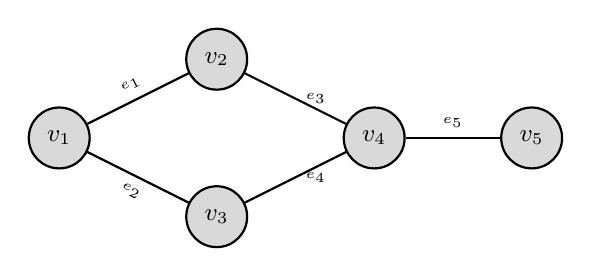
\begin{tikzpicture}[>=Stealth, node distance=1.8cm]
    % Vertices
    \node[vertex] (v1) at (0,0)   {$v_1$};
    \node[vertex] (v2) at (2,1)   {$v_2$};
    \node[vertex] (v3) at (2,-1)  {$v_3$};
    \node[vertex] (v4) at (4,0)   {$v_4$};
    \node[vertex] (v5) at (6,0)   {$v_5$};
    % Edges
    \draw[edge] (v1) -- node[above, sloped, font=\tiny] {$e_1$} (v2);
    \draw[edge] (v1) -- node[below, sloped, font=\tiny] {$e_2$} (v3);
    \draw[edge] (v2) -- node[right, font=\tiny] {$e_3$} (v4);
    \draw[edge] (v3) -- node[right, font=\tiny] {$e_4$} (v4);
    \draw[edge] (v4) -- node[above, font=\tiny] {$e_5$} (v5);
  \end{tikzpicture}
  \caption{A simple graph \(G\) on five vertices and five edges, as described
           in Example~\ref{ex:simple-graph}.  Edge labels \(e_1,\ldots,e_5\)
           are shown for reference.}
  \label{fig:simple-graph}
\end{figure}

\begin{example}[A Directed Graph]\label{ex:digraph}
  Consider the digraph \(D = (V,A)\) with
  \(V = \{u_1, u_2, u_3, u_4\}\) and
  \(A = \{(u_1,u_2),(u_2,u_3),(u_3,u_1),(u_1,u_4),(u_4,u_3)\}\).
  This digraph is depicted in Figure~\ref{fig:digraph}.
  We observe \(\indeg{u_1} = 1\), \(\outdeg{u_1} = 2\).
\end{example}

\begin{figure}[htbp]
  \centering
  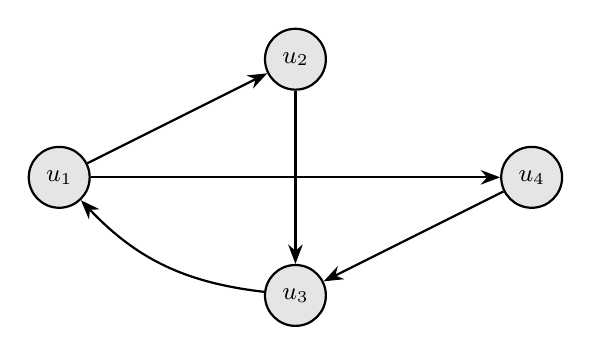
\begin{tikzpicture}[>=Stealth]
    \node[dirvertex] (u1) at (0,0)   {$u_1$};
    \node[dirvertex] (u2) at (3,1.5) {$u_2$};
    \node[dirvertex] (u3) at (3,-1.5){$u_3$};
    \node[dirvertex] (u4) at (6,0)   {$u_4$};
    % Arcs
    \draw[diredge] (u1) -- (u2);
    \draw[diredge] (u2) -- (u3);
    \draw[diredge] (u3) to[bend left=20] (u1);
    \draw[diredge] (u1) -- (u4);
    \draw[diredge] (u4) -- (u3);
  \end{tikzpicture}
  \caption{A directed graph (digraph) \(D\) on four vertices and five arcs,
           as described in Example~\ref{ex:digraph}.}
  \label{fig:digraph}
\end{figure}

%% ============================================================
\section{Basic Properties of Graphs}
\label{sec:properties}
%% ============================================================

\subsection{The Handshaking Lemma}

\begin{theorem}[Handshaking Lemma]\label{thm:handshake}
  Let \(G = (V,E)\) be a simple graph.  Then
  \begin{equation}
    \sum_{v \in V} \dg{v} = 2|E|.
    \label{eq:handshake}
  \end{equation}
\end{theorem}

\begin{proof}
  Each edge \(e = \{u,v\} \in E\) is incident to exactly two vertices,
  namely \(u\) and \(v\).  Therefore, when summing the degrees over all
  vertices, every edge is counted exactly twice — once for each of its two
  endpoints.  Formally, by interchanging the order of summation:
  \begin{align}
    \sum_{v \in V} \dg{v}
    &= \sum_{v \in V} \bigl|\{e \in E : v \in e\}\bigr|
     = \sum_{e \in E} \bigl|\{v \in V : v \in e\}\bigr|
     = \sum_{e \in E} 2
     = 2|E|. \label{eq:handshake-proof}
  \end{align}
\end{proof}

\begin{corollary}\label{cor:odd-degree}
  In any graph \(G = (V,E)\), the number of vertices of odd degree is even.
\end{corollary}

\begin{proof}
  Partition \(V\) into \(V_{\mathrm{odd}} = \{v \in V : \dg{v} \text{ is odd}\}\)
  and \(V_{\mathrm{even}} = V \setminus V_{\mathrm{odd}}\).  By
  Theorem~\ref{thm:handshake},
  \begin{equation}
    \sum_{v \in V_{\mathrm{odd}}} \dg{v}
    + \sum_{v \in V_{\mathrm{even}}} \dg{v} = 2|E|.
    \label{eq:cor-proof}
  \end{equation}
  The right-hand side and the second summand on the left are both even,
  hence \(\sum_{v \in V_{\mathrm{odd}}} \dg{v}\) is even.  Since each term
  in this sum is odd, the number of terms \(|V_{\mathrm{odd}}|\) must be
  even.
\end{proof}

\subsection{Special Vertices}

\begin{definition}[Isolated, Pendant, and Dominating Vertices]
\label{def:special-vertices}
  Let \(G = (V,E)\) be a graph.
  \begin{itemize}
    \item A vertex \(v \in V\) is \emph{isolated} if \(\dg{v} = 0\), i.e.\
          \(\N{v} = \emptyset\).
    \item A vertex \(v \in V\) is a \emph{pendant vertex} (or \emph{leaf})
          if \(\dg{v} = 1\).
    \item A vertex \(v \in V\) is \emph{dominating} if
          \(\Nc{v} = V\), i.e.\ \(v\) is adjacent to every other vertex.
  \end{itemize}
\end{definition}

\subsection{Walks, Trails, Paths, and Cycles}

\begin{definition}[Walk]\label{def:walk}
  A \emph{walk} of \emph{length} \(k\) in a graph \(G = (V,E)\) is a
  finite sequence
  \begin{equation}
    W = v_0,\, e_1,\, v_1,\, e_2,\, v_2,\, \ldots,\, e_k,\, v_k,
    \label{eq:walk}
  \end{equation}
  where \(v_i \in V\) for each \(i\) and \(e_j = \{v_{j-1}, v_j\} \in E\)
  for each \(j\).  The walk is \emph{closed} if \(v_0 = v_k\).
\end{definition}

\begin{definition}[Trail and Path]\label{def:trail-path}
  Let \(W\) be a walk as in Definition~\ref{def:walk}.
  \begin{itemize}
    \item \(W\) is a \emph{trail} if all edges \(e_1, \ldots, e_k\) are
          distinct.
    \item \(W\) is a \emph{path} if additionally all vertices
          \(v_0, v_1, \ldots, v_k\) are distinct.  A path from \(u\) to
          \(v\) is denoted \(u\text{-}v\) path.
  \end{itemize}
\end{definition}

\begin{definition}[Cycle]\label{def:cycle}
  A \emph{cycle} of length \(k \ge 3\) is a closed walk
  \(v_0, e_1, v_1, \ldots, e_k, v_0\) in which all edges are distinct and
  all vertices \(v_0, v_1, \ldots, v_{k-1}\) are distinct.  A cycle of
  length \(k\) is denoted \(C_k\).
\end{definition}

\subsection{Connectedness and Components}

\begin{definition}[Connected Graph]\label{def:connected}
  A graph \(G = (V,E)\) is \emph{connected} if for every pair of distinct
  vertices \(u, v \in V\) there exists a \(u\text{-}v\) path in \(G\).
  Otherwise \(G\) is \emph{disconnected}.
\end{definition}

\begin{definition}[Connected Component]\label{def:component}
  A \emph{connected component} of a graph \(G\) is a maximal connected
  subgraph of \(G\).  Every graph is the disjoint union of its connected
  components.
\end{definition}

\subsection{Subgraphs}

\begin{definition}[Subgraph]\label{def:subgraph}
  A graph \(H = (V', E')\) is a \emph{subgraph} of \(G = (V,E)\),
  written \(H \subseteq G\), if \(V' \subseteq V\) and \(E' \subseteq E\).
  \begin{itemize}
    \item \(H\) is a \emph{spanning subgraph} of \(G\) if \(V' = V\)
          (the vertex set is preserved).
    \item \(H\) is the \emph{subgraph induced} by \(S \subseteq V\),
          written \(G[S]\), if \(V' = S\) and
          \(E' = \{\{u,v\} \in E : u,v \in S\}\)
          (all edges of \(G\) with both endpoints in \(S\) are retained).
  \end{itemize}
\end{definition}

\subsection{Illustrative Example: Paths and Cycles}

\begin{example}[Path and Cycle]\label{ex:path-cycle}
  Figure~\ref{fig:path-cycle} illustrates a graph \(G\) on six vertices
  containing both a highlighted path \(P = v_1, v_2, v_3, v_4\) (shown in
  blue) and a highlighted cycle \(C = v_3, v_4, v_5, v_6, v_3\) (shown in
  red).
\end{example}

\begin{figure}[htbp]
  \centering
  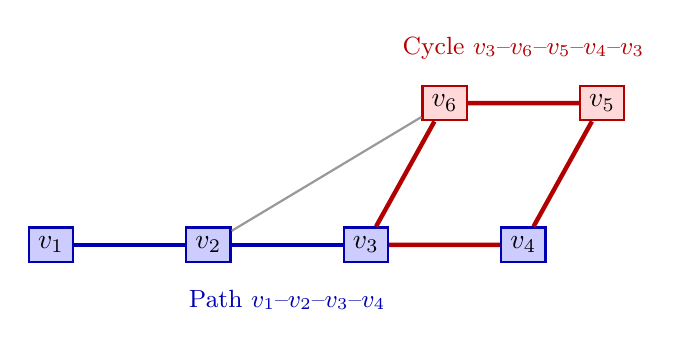
\begin{tikzpicture}[>=Stealth]
    % All vertices
    \node[highlight]  (v1) at (0,0)   {$v_1$};
    \node[highlight]  (v2) at (2,0)   {$v_2$};
    \node[highlight]  (v3) at (4,0)   {$v_3$};
    \node[highlight]  (v4) at (6,0)   {$v_4$};
    \node[cyclehl]    (v5) at (7,1.8) {$v_5$};
    \node[cyclehl]    (v6) at (5,1.8) {$v_6$};
    % Path edges (blue)
    \draw[edge, blue!70!black, line width=1.6pt]
      (v1) -- (v2) -- (v3) -- (v4);
    % Cycle edges (red)
    \draw[edge, red!70!black, line width=1.6pt]
      (v3) -- (v6) -- (v5) -- (v4) -- (v3);
    % Extra edge not on path/cycle
    \draw[edge, black!40] (v6) -- (v2);
    % Legend
    \node[font=\small, blue!70!black] at (3,-0.7)
      {Path $v_1$--$v_2$--$v_3$--$v_4$};
    \node[font=\small, red!70!black]  at (6,2.5)
      {Cycle $v_3$--$v_6$--$v_5$--$v_4$--$v_3$};
  \end{tikzpicture}
  \caption{A graph illustrating a path (blue) and a cycle (red) sharing
           the edge \(\{v_3,v_4\}\), as described in
           Example~\ref{ex:path-cycle}.}
  \label{fig:path-cycle}
\end{figure}

\begin{remark}\label{rem:path-cycle}
  Every cycle \(C_k\) (\(k \ge 3\)) is a connected graph in which every
  vertex has degree exactly \(2\).  Conversely, a connected graph in which
  every vertex has degree \(2\) is a cycle.
\end{remark}

%% ============================================================
\section{Graph Isomorphism}
\label{sec:isomorphism}
%% ============================================================

\subsection{Motivation}

Two graphs may appear different — possessing distinct vertex labels or
geometric representations — yet share an identical abstract structure.  The
notion of \emph{graph isomorphism} makes this intuition precise by requiring
the existence of a structure-preserving bijection between vertex sets.

\begin{remark}\label{rem:iso-motivation}
  When studying graph-theoretic properties (connectivity, degree sequences,
  cycle lengths, etc.), the actual names of vertices are irrelevant.  Two
  isomorphic graphs satisfy exactly the same graph-theoretic statements.
\end{remark}

\subsection{Formal Definition}

\begin{definition}[Graph Isomorphism]\label{def:isomorphism}
  Two graphs \(G_1 = (V_1, E_1)\) and \(G_2 = (V_2, E_2)\) are
  \emph{isomorphic}, written \(G_1 \cong G_2\), if there exists a bijection
  \begin{equation}
    f : V_1 \longrightarrow V_2
    \label{eq:bijection}
  \end{equation}
  such that for all \(u, v \in V_1\),
  \begin{equation}
    \{u,v\} \in E_1 \iff \{f(u),\, f(v)\} \in E_2.
    \label{eq:iso-condition}
  \end{equation}
  Such a bijection \(f\) is called an \emph{isomorphism} from \(G_1\) to
  \(G_2\).
\end{definition}

\begin{remark}\label{rem:iso-equivalence}
  Graph isomorphism is an equivalence relation on the class of all graphs:
  it is reflexive (the identity map is always an isomorphism
  \(G \cong G\)), symmetric (if \(f\) is an isomorphism \(G_1 \to G_2\)
  then \(f^{-1}\) is an isomorphism \(G_2 \to G_1\)), and transitive
  (the composition of two isomorphisms is an isomorphism).
\end{remark}

\subsection{Graph Invariants}

A \emph{graph invariant} is a property that takes the same value on
isomorphic graphs.  Invariants provide a practical tool for proving
non-isomorphism: if two graphs differ on any invariant, they cannot be
isomorphic.

\begin{definition}[Graph Invariants]\label{def:invariants}
  The following are well-known graph invariants:
  \begin{enumerate}
    \item \textbf{Order and size:} \(|V|\) and \(|E|\).
    \item \textbf{Degree sequence:} the non-decreasing sequence of vertex
          degrees (Definition~\ref{def:degseq}).
    \item \textbf{Cycle spectrum:} the set of lengths of cycles present in
          the graph.
    \item \textbf{Connectivity:} whether the graph is connected; the number
          of connected components.
    \item \textbf{Diameter:} \(\mathrm{diam}(G) = \max_{u,v \in V} d(u,v)\),
          where \(d(u,v)\) denotes the length of a shortest \(u\)-\(v\) path.
  \end{enumerate}
\end{definition}

\begin{theorem}[Necessary Conditions for Isomorphism]\label{thm:iso-necessary}
  If \(G_1 \cong G_2\) via isomorphism \(f\), then:
  \begin{enumerate}
    \item \(|V_1| = |V_2|\) and \(|E_1| = |E_2|\),
    \item \(G_1\) and \(G_2\) have the same degree sequence,
    \item \(G_1\) is connected if and only if \(G_2\) is connected.
  \end{enumerate}
\end{theorem}

\begin{proof}
  Since \(f: V_1 \to V_2\) is a bijection, \(|V_1| = |V_2|\).  Because
  \(f\) preserves adjacency (equation~\eqref{eq:iso-condition}), it
  induces a bijection on edge sets, whence \(|E_1| = |E_2|\).  For
  each vertex \(v \in V_1\), adjacency-preservation implies
  \(\deg_{G_1}(v) = \deg_{G_2}(f(v))\), so the degree sequences coincide.
  Connectivity is preserved because \(f\) maps paths in \(G_1\) to paths
  in \(G_2\).
\end{proof}

\begin{remark}\label{rem:sufficient}
  The conditions in Theorem~\ref{thm:iso-necessary} are \emph{necessary}
  but not \emph{sufficient}.  Two graphs may share the same order, size,
  and degree sequence while failing to be isomorphic.  Determining whether
  two graphs are isomorphic is a computationally challenging problem (graph
  isomorphism lies in \(\mathsf{NP}\) and is not known to be
  \(\mathsf{NP}\)-complete).
\end{remark}

\subsection{Examples}

\begin{example}[Two Isomorphic Graphs]\label{ex:iso}
  The graphs \(G_1\) and \(G_2\) depicted in Figure~\ref{fig:isomorphic}
  are isomorphic.  Both have order \(4\), size \(4\), and degree sequence
  \((2,2,2,2)\).  The isomorphism
  \begin{equation}
    f(a_1)=b_1,\quad f(a_2)=b_2,\quad f(a_3)=b_3,\quad f(a_4)=b_4
    \label{eq:iso-map}
  \end{equation}
  witnesses \(G_1 \cong G_2\), as may be verified by checking that each
  edge of \(G_1\) maps to an edge of \(G_2\) and vice versa.
\end{example}

\begin{figure}[htbp]
  \centering
  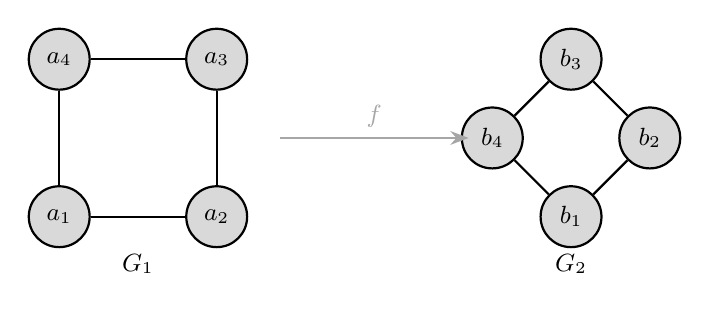
\begin{tikzpicture}[>=Stealth]
    %% G1: cycle a1-a2-a3-a4-a1 (square layout)
    \begin{scope}[xshift=0cm]
      \node[vertex] (a1) at (0,0)   {$a_1$};
      \node[vertex] (a2) at (2,0)   {$a_2$};
      \node[vertex] (a3) at (2,2)   {$a_3$};
      \node[vertex] (a4) at (0,2)   {$a_4$};
      \draw[edge] (a1)--(a2)--(a3)--(a4)--(a1);
      \node[font=\itshape\small] at (1,-0.6) {$G_1$};
    \end{scope}
    %% G2: cycle b1-b2-b3-b4-b1 (diamond layout)
    \begin{scope}[xshift=5.5cm]
      \node[vertex] (b1) at (1,0)   {$b_1$};
      \node[vertex] (b2) at (2,1)   {$b_2$};
      \node[vertex] (b3) at (1,2)   {$b_3$};
      \node[vertex] (b4) at (0,1)   {$b_4$};
      \draw[edge] (b1)--(b2)--(b3)--(b4)--(b1);
      \node[font=\itshape\small] at (1,-0.6) {$G_2$};
    \end{scope}
    %% Isomorphism arrow
    \draw[-{Stealth}, thick, gray!70]
      (2.8,1) -- node[above, font=\small\itshape]{$f$} (5.2,1);
  \end{tikzpicture}
  \caption{Two isomorphic graphs \(G_1 \cong G_2\) (both are \(C_4\)) with
           different vertex labels and geometric embeddings, as described in
           Example~\ref{ex:iso}.}
  \label{fig:isomorphic}
\end{figure}

\begin{example}[Two Non-Isomorphic Graphs]\label{ex:noniso}
  The graphs \(H_1\) and \(H_2\) depicted in Figure~\ref{fig:nonisomorphic}
  both have order \(4\) and size \(4\).  However, their degree sequences
  differ:
  \begin{align}
    \text{degree sequence of } H_1 &= (1,1,2,4), \label{eq:degseq-H1}\\
    \text{degree sequence of } H_2 &= (2,2,2,2). \label{eq:degseq-H2}
  \end{align}
  By Theorem~\ref{thm:iso-necessary}, \(H_1 \not\cong H_2\).
\end{example}

\begin{figure}[htbp]
  \centering
  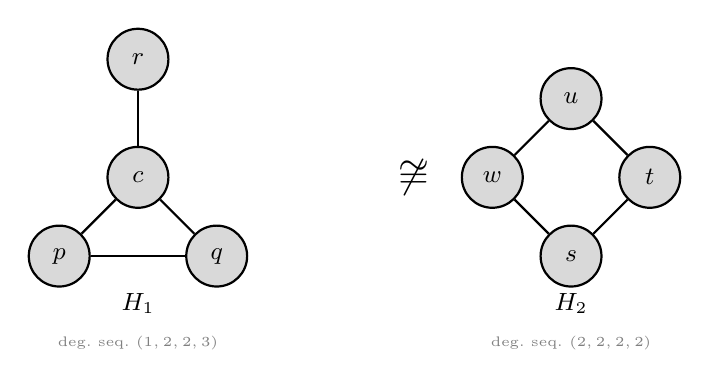
\begin{tikzpicture}[>=Stealth]
    %% H1: star K_{1,3} plus one extra edge giving a high-degree vertex
    \begin{scope}[xshift=0cm]
      % Central vertex c has degree 3; add edge between two leaves to get (1,1,2,3)
      % Actually: let's make a "lollipop"-style graph
      % v1 connected to v2,v3,v4 and v2-v3 edge → degrees: v1=3,v2=2,v3=2,v4=1
      % Use: path v4-v1-v2-v3-v1 → degrees: v1=3,v2=2,v3=2,v4=1 → seq (1,2,2,3)
      \node[vertex] (h1v1) at (1,1)   {$c$};
      \node[vertex] (h1v2) at (0,0)   {$p$};
      \node[vertex] (h1v3) at (2,0)   {$q$};
      \node[vertex] (h1v4) at (1,2.5) {$r$};
      \draw[edge] (h1v1)--(h1v2);
      \draw[edge] (h1v1)--(h1v3);
      \draw[edge] (h1v1)--(h1v4);
      \draw[edge] (h1v2)--(h1v3);
      \node[font=\itshape\small] at (1,-0.6) {$H_1$};
      \node[font=\tiny, gray] at (1,-1.1) {deg.\ seq.\ $(1,2,2,3)$};
    \end{scope}
    %% H2: 4-cycle (all degrees 2)
    \begin{scope}[xshift=5.5cm]
      \node[vertex] (h2v1) at (1,0)   {$s$};
      \node[vertex] (h2v2) at (2,1)   {$t$};
      \node[vertex] (h2v3) at (1,2)   {$u$};
      \node[vertex] (h2v4) at (0,1)   {$w$};
      \draw[edge] (h2v1)--(h2v2)--(h2v3)--(h2v4)--(h2v1);
      \node[font=\itshape\small] at (1,-0.6) {$H_2$};
      \node[font=\tiny, gray] at (1,-1.1) {deg.\ seq.\ $(2,2,2,2)$};
    \end{scope}
    %% Non-isomorphism marker
    \node[font=\Large] at (4.5,1) {$\not\cong$};
  \end{tikzpicture}
  \caption{Two non-isomorphic graphs \(H_1 \not\cong H_2\) on four vertices
           and four edges, distinguished by their degree sequences
           (see Example~\ref{ex:noniso}).}
  \label{fig:nonisomorphic}
\end{figure}

\begin{remark}\label{rem:iso-hardness}
  Although the degree sequence is a convenient invariant for refuting
  isomorphism (as in Example~\ref{ex:noniso}), no finite set of polynomial-time
  invariants is known that \emph{decides} isomorphism for all graphs.  The
  graph isomorphism problem remains one of the most intriguing open problems
  at the interface of combinatorics and computational complexity.
\end{remark}

\end{document}